\newpage
\section{Auswertung}
\label{sec:Auswertung}

\subsection{Temperaturverläufe}
    Die Temperaturverläufe in Abbildung \ref{fig:plot_temp} dargestellt
    \begin{figure}
        \centering
        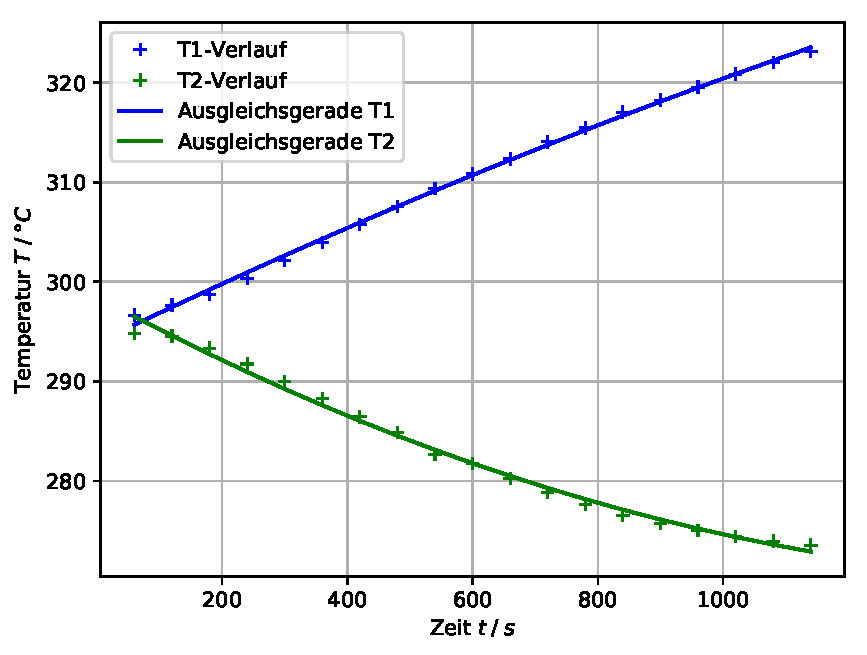
\includegraphics[width=\textwidth]{build/plot_temp.pdf}
        \caption{Temperaturverläufe}
        \label{fig:plot_temp}
    \end{figure}

\subsection{Nicht-lineare Ausgleichsrechnung}
    Mit der folgenden Näherung, werden nun die in \ref{fig:plot_temp}
    dargestellten Ausgleichsgeraden bestimmt\cite{curvefit}:
    \begin{equation}
        T(t)=At^2+Bt+C
        \label{eqn:ausgleichsgerade}
    \end{equation}
    \begin{table}
        \centering
        \begin{tabular}{c || c | c}
            \toprule
            & $T_1\;/\;K$ & $T_2\;/\;K$ \\
            \midrule
            A\;/\;$K/s^2$& $(-3.8\pm0.9)\;10^{-6}$ & $(1.01\pm0.16)\;10^{-5}$ \\
            B\;/\;$K/s$& 0.0304\pm0.0012 & -0.0339\pm0.0019 \\
            C\;/\;$K$& 293.88\pm0.30 & 298.5\pm0.5 \\
            \bottomrule
        \end{tabular}
    \end{table}
\subsection{Differentialquotienten}
    Exemplarisch werden für vier Messwerte der Differentialquotienten $dT1/dt$ und
    $dT2/dt$ berechnet.
    Für die Näherung von \eqref{eqn:ausgleichsgerade} folgt somit:
    \begin{equation}
        \frac{dT}{dt}=2At+Bt
    \end{equation}
    
    \begin{table}
        \centering
        \begin{tabular}{c c c}
            \toprule
            Zeit $T\;/\;s$ & $T_1$ & d$T_1$/d$t$ \\
            \midrule
            240,0 & 300,35 & 0.0285\pm0.0012\\
            480,0 & 307,55 & 0.0267\pm0.0015 \\
            840,0 & 317,045 & 0.0239\pm0.0020  \\
            1080,0 & 322,045 & 0.0221\pm0.0023\\
            \midrule
            Mittelwert &&  0.0253\pm0.0017  \\
            \bottomrule
        \end{tabular}
        \caption{Differentialquotienten für $T_1$}
        \label{fig:tab_T1t}
    \end{table}

    \begin{table}
        \centering
        \begin{tabular}{c c c c}
            \toprule
            Zeit $T\;/\;s$ & $T_2$ & d$T_2$/d$t$ \\
            \midrule
            240.0 & 291.75 & -0.029 \\
            480.0 & 284.85 & -0.024 \\
            840.0 & 276.55 & -0.017 \\
            1080.0 & 273.95 & -0.012 \\
            \midrule
            Mittelwert &&  -0,021 \\
            \bottomrule
        \end{tabular}
        \caption{Differentialquotienten für $T_2$}
        \label{fig:tab_T2t}
    \end{table}
    \newpage
    \subsection{Bestimmung der Güteziffer}
    Wie in Gleichung (\ref{eqn:nu_ideal}) dargestellt, lässt sich aus dem zuvor berechneten
    Differentialquotienten die Güteziffer $\nu$ bestimmen.\\
    Für die Wärmekapazität von Wasser $m_1\;c_w$ und von Kupfer $m_k\;c_k$ gilt gilt \cite{wasser}:
    \begin{align*}
        m_1\;c_w &= 4190\frac{J}{kg\;K} 	\Rightarrow 12570\frac{J}{K}\\
        m_k\;c_k &= 750\frac{J}{K}
    \end{align*}

    \begin{table}
        \centering
        \begin{tabular}{c c c}
        \toprule
        Zeit $t\;/\;s$ & Güteziffer $v_{ideal}$ & Güteziffer $v_{real}$  \\
        \midrule
        120.0 & 96.02 & 1.97\pm0.08 \\
        480.0 & 24.77 & 1.87\pm0.09 \\
        840.0 & 7.83 & 1.60\pm0.13 \\
        1140.0 & 6.56 & 1.45\pm0.16 \\
        \end{tabular}
    \end{table}
    
%%%%%%%%%%%%%%%%%%%%%%%%%%%%%%%%%%%%%%%%%%%%%%%%%%%%%%%%%

\subsection{Massendurchsatz}
Zuerst wird die Verdampfungswärme mithilfe einer linearen Regression wie in Versuch 203 bestimmt.

\begin{figure}
  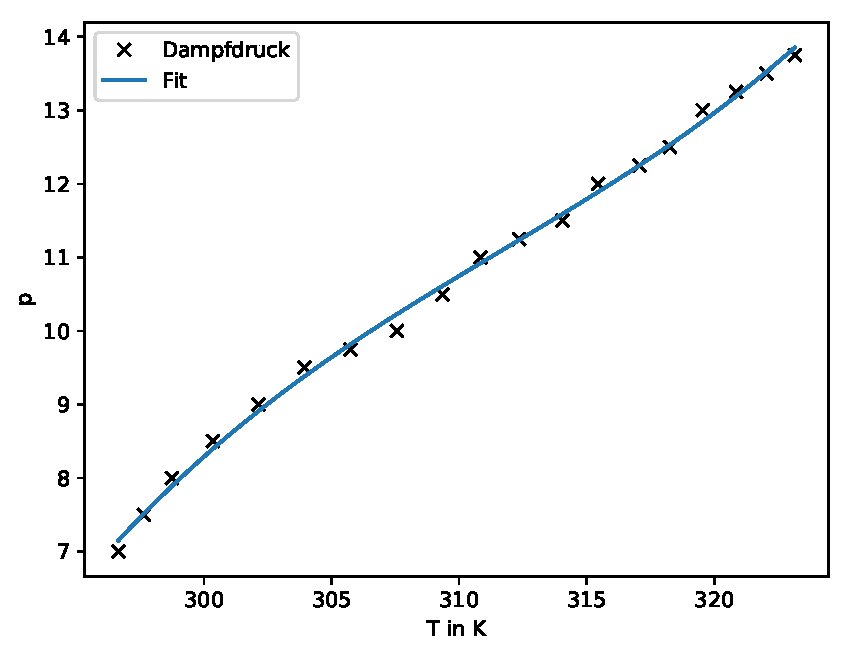
\includegraphics{build/plot_L.pdf}
  \caption{Dampfdruckkurve für $\symup{P}$ und $\symup{T}$ im warmen Reservoir.}
  \label{fig:Dampfp}
\end{figure}

Es wird eine Ausgleichsrechnung mit
\begin{equation}
  f(x)= Ax^3+Bx^2+Cx+D
\end{equation}
Wobei $A, B , C$ und $D$ die Koeffizienten der Rechnung sind.
\\
Die Paramter der linearen Ausgleichsrechnung ergeben sich zu
\begin{align*}
  \symup{A} &= \SI{17721.75 \pm 1000.48}{\kelvin} \\
  \symup{B} &= \num{9.29(39)} \\
  \symup{C} &= \num{9.29(39)} \\
  \symup{D} &= \num{9.29(39)} \:
\end{align*}
\\
Die Unsicherheit ergibt sich mit der Gauß'schen Fehlerfortpflanzung nach
\begin{equation}
  \increment \symup{L} = \frac{1}{M} \increment \symup{A}
  \label{eqn:gauss}
\end{equation}
Mit dem so erhaltenen Wert für $L$ wird nun der Massendurchsatz bestimmt.
Der Massendurchsatz $\symup{d}m / \symup{d}t$ an der jeweiligen Messstelle ist
in Tabelle \ref{tab:massendurch} aufgeführt.
\begin{table}
        \centering
        \begin{tabular}{c c}
        \toprule
        Zeit $t\;/\;s$ & Massendurchsatz in kg/s \\
        \midrule
        240.0 & (0.0002 \pm 9.9347) $ 10^{-6}$\\
        480.0 & (0.0001 \pm 8.14441)$ 10^{-6}$ \\
        840.0 & ( 0.0001\pm 1.0285) $10^{-5}$\\
        1080.0 & (0.0001\pm 1.1958) $10^{-5}$\\
        \end{tabular}
        \caption{Massendurchsatz}
        \label{tab:massendurch}
    \end{table}

Die Unsicherheiten entstehen wieder nach Gaußfehler \ref{eqn:gauss}.
Für $\increment \dot{m}$ gilt dann
\begin{equation}
  \increment \dot{m} = \frac{1}{L} \sqrt{\dot{Q}_\text{kalt}^2 (\increment L)^2
  + (\increment \dot{Q}_\text{kalt})^2}
\end{equation}

\subsection{Mechanische Kompressionsleistung}
Die mechanische Kompressionsleistung bestimmt sich über \ref{eqn:kompress} und \ref{eqn:kompress2}
\begin{equation}
    \increment \dot{m} = -0.00390 \pm 0.00017
\end{equation}